\begin{savequote}
	Free as in speech (freedom), not as in free beer
\qauthor{Richard Stallman}
\end{savequote}

\chapter{Antes de leer estas paginas}
\section{Aviso}
\begin{mdframed}[backgroundcolor=yellow]
	
\includegraphics[width=0.05\textwidth]{figures/warning.png}
	El contenido que vas a leer a continuacion puede resultar politicamente incorrecto dependiendo del lugar/epoca en la que estes leyendo esto
	
\includegraphics[width=0.05\textwidth]{figures/warning.png}
\end{mdframed}
\section{Motivacion para la lectura}
Mucha gente vive su vida viendola pasar, como si su vida fuera un avion que pasa por encima de ellos sin que puedan hacer nada para modificar su rumbo, que ha sido prestablecidode inicio a fin. Pero la realidad es muy distinta, y es que vamos a pie, en cualquier momento podemos dar un giro de 180 grados, solo necesitamos la fuerza para luchar contra lo que venga.\\

Sientes con frecuencia que tienes comportamientos diferentes segun con el grupo de personas que estes? Eres una persona a veces y otras veces otra? \\
Cuando estas con gente, haces cosas que normalmente no harias para sentir que perteneces al grupo? \\
Si en un grupo, los demas estan haciendo algo que no te apetece, como te sientes? \\
Tienes alguna meta clara en la vida, persigues algun objetivo? Es posible que te hayas propuesto algo por influencia de los demas sin pararte a pensar si realmente es lo que quieres? \\
Cuando tomas decisiones que tienes en cuenta? Te frena \textit{el que diran} cuando estas pasando por el camino hacia tus metas?\\
Cuando te pasa algo, como una situacion sobrevenida negativa que no te esperabas, eres capaz de reaccionar ante ella para salir mas fuerte o culpas a agentes externos?\\
Si alguna de las anteriores preguntas te ha chocado o te ha hecho pensar, te animo a seguir leyendo y descubrir cosas nuevas. \\

Es cierto que vivimos en sociedad y que negarse a ello seria luchar contra la naturaleza, pero hay sociedades en las que los individuos no son por si mismos, solo en sociedad. Las metas que se han establecido son probablemente impuestas por los estandares de la sociedad sin pararse a reflexionar. De esta forma, en ocasiones, el motivo de su vida es esa sociedad.
Yo mismo he podido ver como gente que tenia una opinion fuerte a cerca de un tema, rompieron su integridad sin pensarlo mucho y como saben que lo que han hecho iba en contra de sus principios, buscan apoyo en la opinion de los demas que les es favorable y asi se justifican. 
\subsection{Historias que invitan a la reflexion}
Esto es lo que me parece mas grave, y pondre un ejemplo, consta de dos personas, que llamaremos \textit{uno} y \textit{dos}:
(Esta historia ha sido ligeramente modificada para estresar el problema que quiero comentar)

Uno ni se planteaba en su vida fumar, era algo contra lo que tenia una opinion fuerte sustentada por si mismo. Uno se mantuvo integro un tiempo, sin embargo yo desde fuera veia que en ocasiones se dejaba llevar un poco en este tema. Ante mis avisos, lo que obtuve fueron reprimendas sociales. El dia llego en el que finalmente tiro este principio por la ventana e hizo lo que dijo que nunca haria. La justificacion fue bastante curiosa, \textit{es que dos se tenia que acabar su cajeta y le sobraban}. Y por supuesto, mientras lo seguia haciendo seguia encontrando justificaciones. Curioso cuanto menos no? 

Es a este tipo de actos, aunque el que he retratado anteriormente es meramente anecdotico y en una escala de peligro es bajo, pues como mucho se hara dano a si mismo, a los que me refiero cuando digo que las sociedades pueden resultar malas (malas en el sentido de que corrompen nuestros principios) si no se tiene la suficiente fuerza para decir no en este caso, o en otras palabras, ser verdaderamente independiente. \\

Pensemos por un segundo en el ejemplo anterior que habria pasado si uno le hubiera dicho a dos que no que no lo haria, que si se los tenia que acabar los podria tirar a la papelera. Uno se habria mantenido integro a sus principios, pero que habria pensado dos? Quizas habria sentido rechazo al ver que uno no cederia, esto en ocasiones en mi experiencia deja ver cierta inseguridad en dos, pues una de sus formas de justificar lo que hace es que lo demas lo hagan, es algo como: \textit{o estas conmigo o estas contra mi} y eso crea una presion fuerte en las relaciones entre personas especialmente en grupo cuando hay \textit{"1 contra N"} \\

En otra historia, voy a tratar de demostrar la falta de independencia no en cuanto a un grupo necesariamente si no en cuanto a un individuo en si mismo, esto fue una conversacion que tuve con un amigo: 

\begin{dialogue}
	\speak{Uno} Vente hoy
	\direct{
		Refiriendose a ir con un grupo de gente a una casa por la noche
		}
	\speak{Dos} Pero que haceis en una casa metidos?
	\speak{Uno} Pues beber y jugar a juegos de mesa
	\speak{Dos} Tu crees que eso es lo mas productivo que puedes hacer?
	\speak{Uno} Es que no hay mucho mas que hacer
	\speak{Uno} Propon tu otra cosa si no!
	\speak{Dos} A ver, haz lo que quieras, pero hay cientos de cosas que podrias estar haciendo que te proporcionaran un mejor futuro. 
	\speak{Uno} De estudiar dices?
	\speak{Dos} Y no necesitas que los demas te propongan cosas para hacer lo que tu realmente quieras.
	\speak{Uno} No solo de estudiar, que tambien, pero de invertir en ti mismo...
	\speak{Dos} Bua, te has rayado.

\end{dialogue}

Y no es que yo quiera criticar a esta persona en concreto, si no que veo que la mayoria de gente de mi generacion sigue este rumbo:

\begin{enumerate}
	\item Esperar a que alguien les proponga algo que hacer
	\item Valorar entre las varias opciones que les han propuesto y cenirse a una sin pararse a pensar si quiera en lo que ellos quieren realmente ni en las consecuencias que va a tener esto en sus vidas a largo plazo, pues en general miran en corto
\end{enumerate}

Por otro lado lo que yo hago es algo asi como lo siguiente:

\begin{enumerate}
	\item Valorar lo que te gustaria conseguir en la vida en un determinado instante de tiempo
	\item Buscar un plan para hacerlo realidad
	\item Ahora sabras cuales son las acciones que tienes que llevar a cabo para hacer realidad tus deseos, y no dependeras de que los demas propongan un plan para "tener algo que hacer"
	\item Esto no quita que algun dia te puedas o no salir de este plan, pero al hacerlo seras plenamente consciente de cuanto te va a retrasar eso de conseguir tu meta o incluso puede que te aleje. Pero ya tendras una forma de medir, una forma de decidir lo que quieres hacer independientemente de los demas
\end{enumerate}
 
\subsection{Por que independencia?}
Mi definicion de independencia:
La independencia es libertad para actuar acorde con los principios que hemos desarrollado por nosotros mismos, que no tienen que ser fijos ni estaticos durante toda la vida, pero tienen que venir de forma genuina de nosotros. Cuando tenemos esta libertad y somos integros con nuestros principios, estaremos completos por nosotros mismos y no necesitaremos de los demas para justificarnos. Las relaciones interpersonales toman otro rumbo mucho mas enriquecedor y puro pues nosotros ahora sabemos quienes somos y podemos ver los puntos de vista de los demas como una experiencia diferente y enriquecedora y no como algo que tenemos que adoptar para ser parte del grupo.
Como hemos visto en la historia anterior, es necesario tener principios claros y muy importante tambien es ser lo suficientemente fuerte para aguantar la presion social y saber decir que no en ese caso, pero la independencia no es solo en lo social, hay otros ambitos importantes.
\subsection{Cual es el minimo grado de independencia?}
Como ya comentaba, y ahora sintetizo, creo que el minimo grado de independencia que uno debe tener es el suficiente para actuar en contra si es necesario de la sociedad o lo que hace la mayoria si asi creemos en ello. No hacer lo que hacen los demas, la imagen mas clara es la del rebano de las ovejas que no saben hacer otra cosa que seguirse las unas a las otras en contraste con el lobo que se vale por si mismo cuando esta solo pero \underline{cuando va con la manada se crece y multiplica sus fuerzas}, esto es, es \textbf{interdependiente}
\subsection{Por que la independencia no es suficiente?}
Como comentaba en el punto anterior con el lobo que es perfectamente capaz de valerse por si mismo sin necesitar de los demas, no sigue al rebano de ovejas, pero como es independiente por si mismo, cuando se junta en manada con otros lobos independientes, juntos son capaces de hacer cosas increibles.
Esto es el paso siguiente a la independencia

\subsection{Mis influencias}
En la introduccion comentaba que cuando estas abierto al cambio es cuando realmente tienes la capacidad de aprender y crecer como persona, y que para ello lo mejor que puedes hacer es leer, atender clases de profesores y rodearte de gente que te enriquece. Esto es muy dificil pues mucha gente tiene segundas intenciones y puede tratar de manipular, sin embargo yo creo que encontre muy buenos apoyos en las siguientes fuentes:
\begin{itemize}
	\item{ \textit{the 7 habits of highly effective people} de Stephen R Covey 
		\begin{figure}[h]
			\centering
			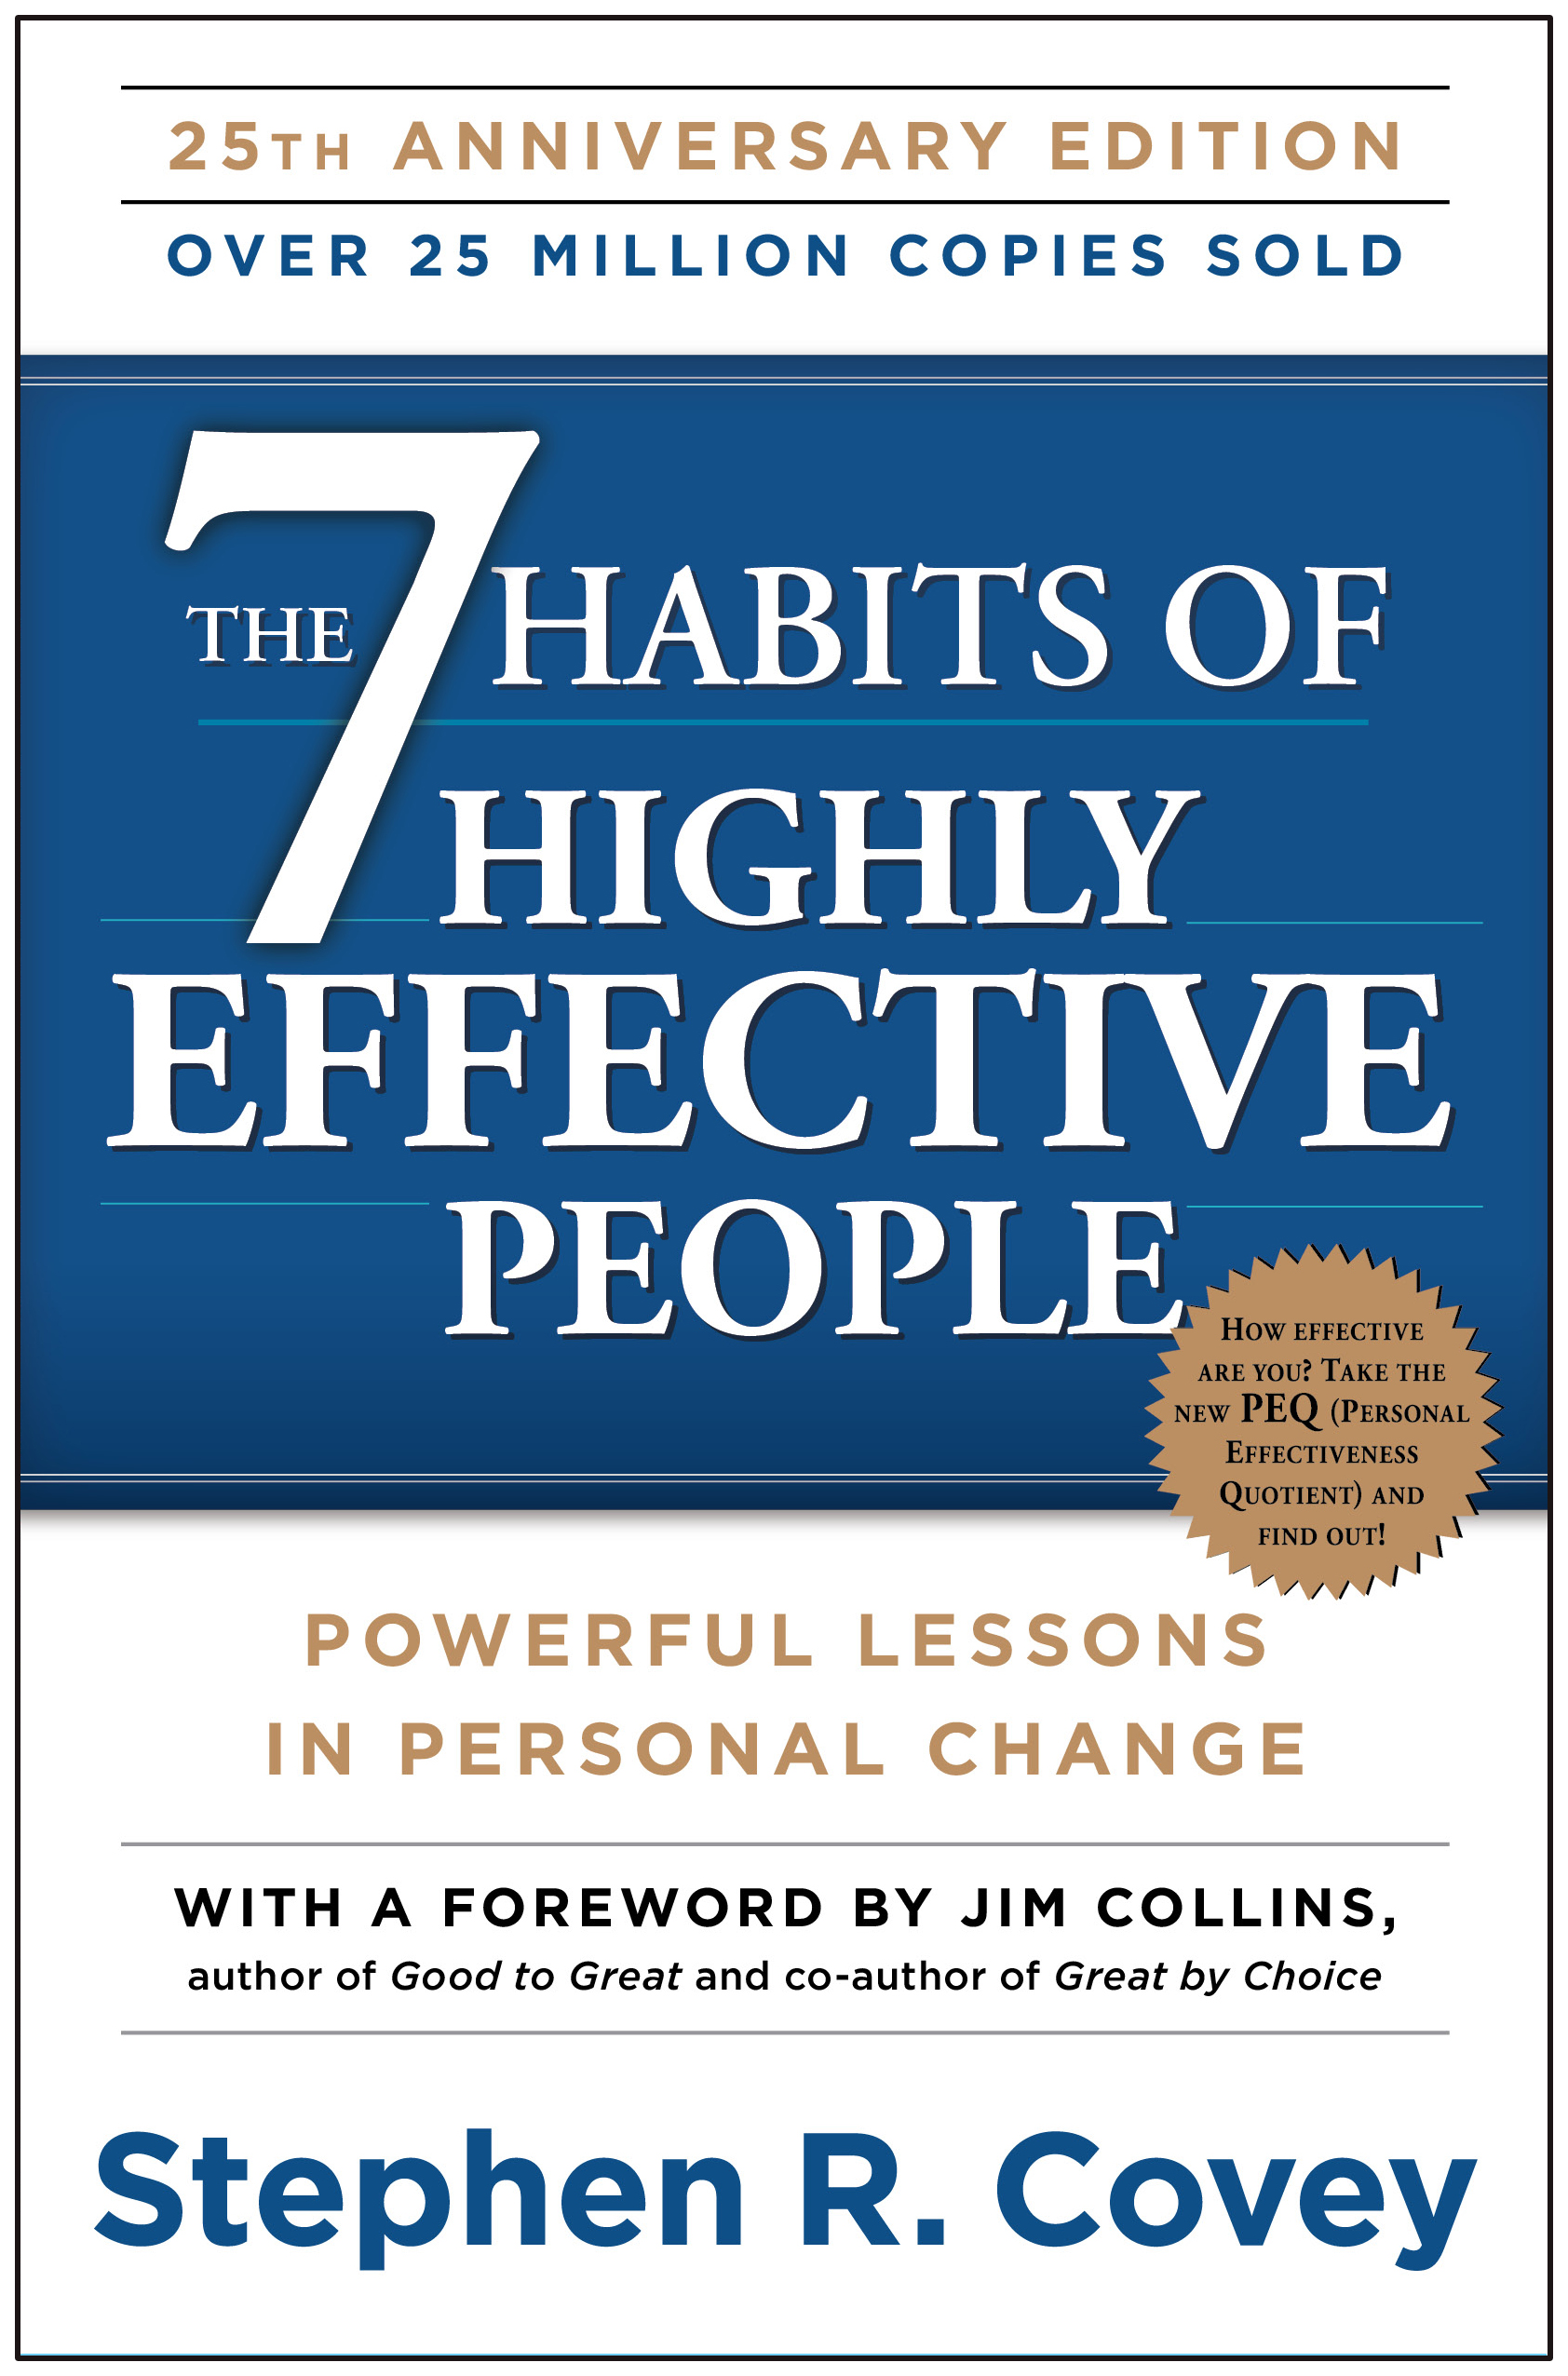
\includegraphics[width=0.4\textwidth]{figures/the7habits.jpg}
			\caption{The 7 habits of highly effective people by Stephen R Covey}
		\end{figure}
	}
\item{ canales de youtube que hablan sobre independencia en el ambito de la informatica: luke smith o distro tube
		\begin{figure}[H]
			\centering
			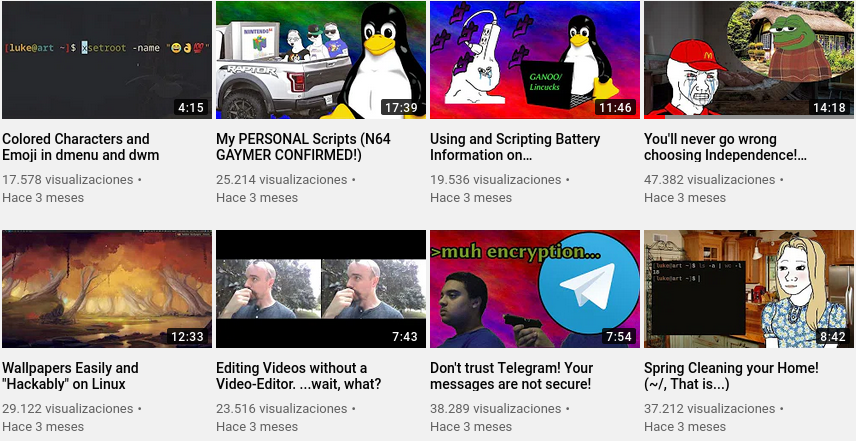
\includegraphics[width=0.75\textwidth]{figures/luke-smith.png}
			\caption{Captura de pantalla de las portadas de algunos videos de luke smith}
		\end{figure}
	}
\item {profesores como juan ramon rallo que apelan a la reflexion sobre las decisiones politicas en nuestro pais dando un punto de vista lleno de datos objetivos (fundamentalmente aboga por la libertad en la economia)
		\begin{figure}[H]
			\centering
			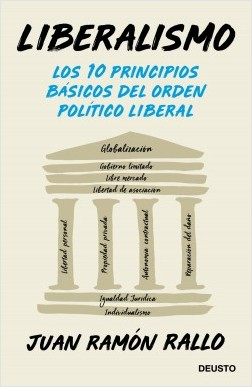
\includegraphics[width=0.5\textwidth]{figures/rallo.jpg}
			\caption{Uno de los libros de juan ramon rallo}
		\end{figure}
		}
\end{itemize}

Estas fuentes no han hecho mas que poner en forma de palabras y ampliar conceptos en los que yo ya creia, es por eso que creo que han sido tan enriquecedoras. No es que lo haya leido y me haya convertido en defensor de la independencia, si no que ya creia y actuaba de forma indpeendiente y luego me tope con estas fuentes que me enriquecieron pues era gente mas sabia que ya habia vivido mucho mas que yo y que me confirmo que no solo es posible recorrer este camino si no que en sus palabras los resultados son maravillosos. Yo creo por tanto que es sabio aprender de gente que tiene los resultados que nosotros queremos alcanzar.

He de comentar que a pesar que las fuentes mencionadas anteriormente han sido muy nutritivas en mi forma de pensar y de ver las cosas, yo ya estaba en ese "mindset". Sin embargo he de dar el mayor de los creditos a una fuente en la que siempre me he apoyado cuando vivia momentos malos, cuando no veia una salida, cuando tenia que tomar una decision y me planteaba venderme a mi mismo, esta se compone de los muchisimos discursos motivacionales de Fearless Motivation, si estas pasando por un mal momento a cualquier nivel, te recomiendo que le eches un vistazo
		\begin{figure}[H]
			\centering
			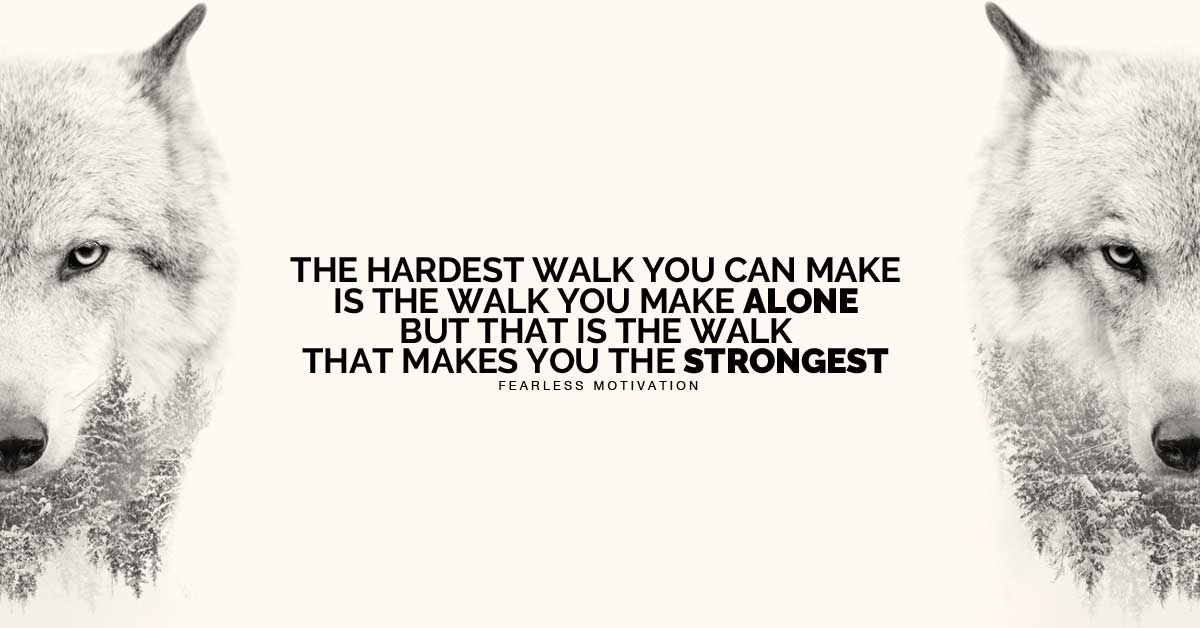
\includegraphics[width=0.75\textwidth]{figures/wolf.jpeg}
			\caption{Una imagen de uno de los videos de fearless motivation}
		\end{figure}


